The \textbf{SpiNNaker} system is a massively-parallel, bio-inspired computing platform. The goal of the project is to build a machine that will contain $\sim$1 million CPU cores and will be able to simulate $\sim$1 billion neurons in real time. As any multi-core system, communication between cores is basic; the SpiNNaker chip has been designed to efficiently implement neural networks, thus, networking is specialized (but not limited) to transmit spikes.

\subsection{SpiNNaker chip overview}

SpiNNaker chips consist of 18 ARM968 cores, each with tightly-coupled program and data memory. Each core also has a Communication Network-on-Chip (C-NoC) interface that, with the help of an in-die network router, allows inter- and intra-chip communications (Figure~\ref{fig:hw:spinnaker-die}). On top of the chip lie 128 MBytes of Synchronous Dynamic RAM (SDRAM) whose die is stitch-bonded to the chip for faster access (Figure~\ref{fig:hw:bonded-sdram}). The SpiNNaker chip plus the SDRAM are sometimes referred as a \emph{node}~\cite{furber2013overview}.

\begin{figure}[h]
  \begin{center}
    \begin{subfigure}[b]{0.55\textwidth}
      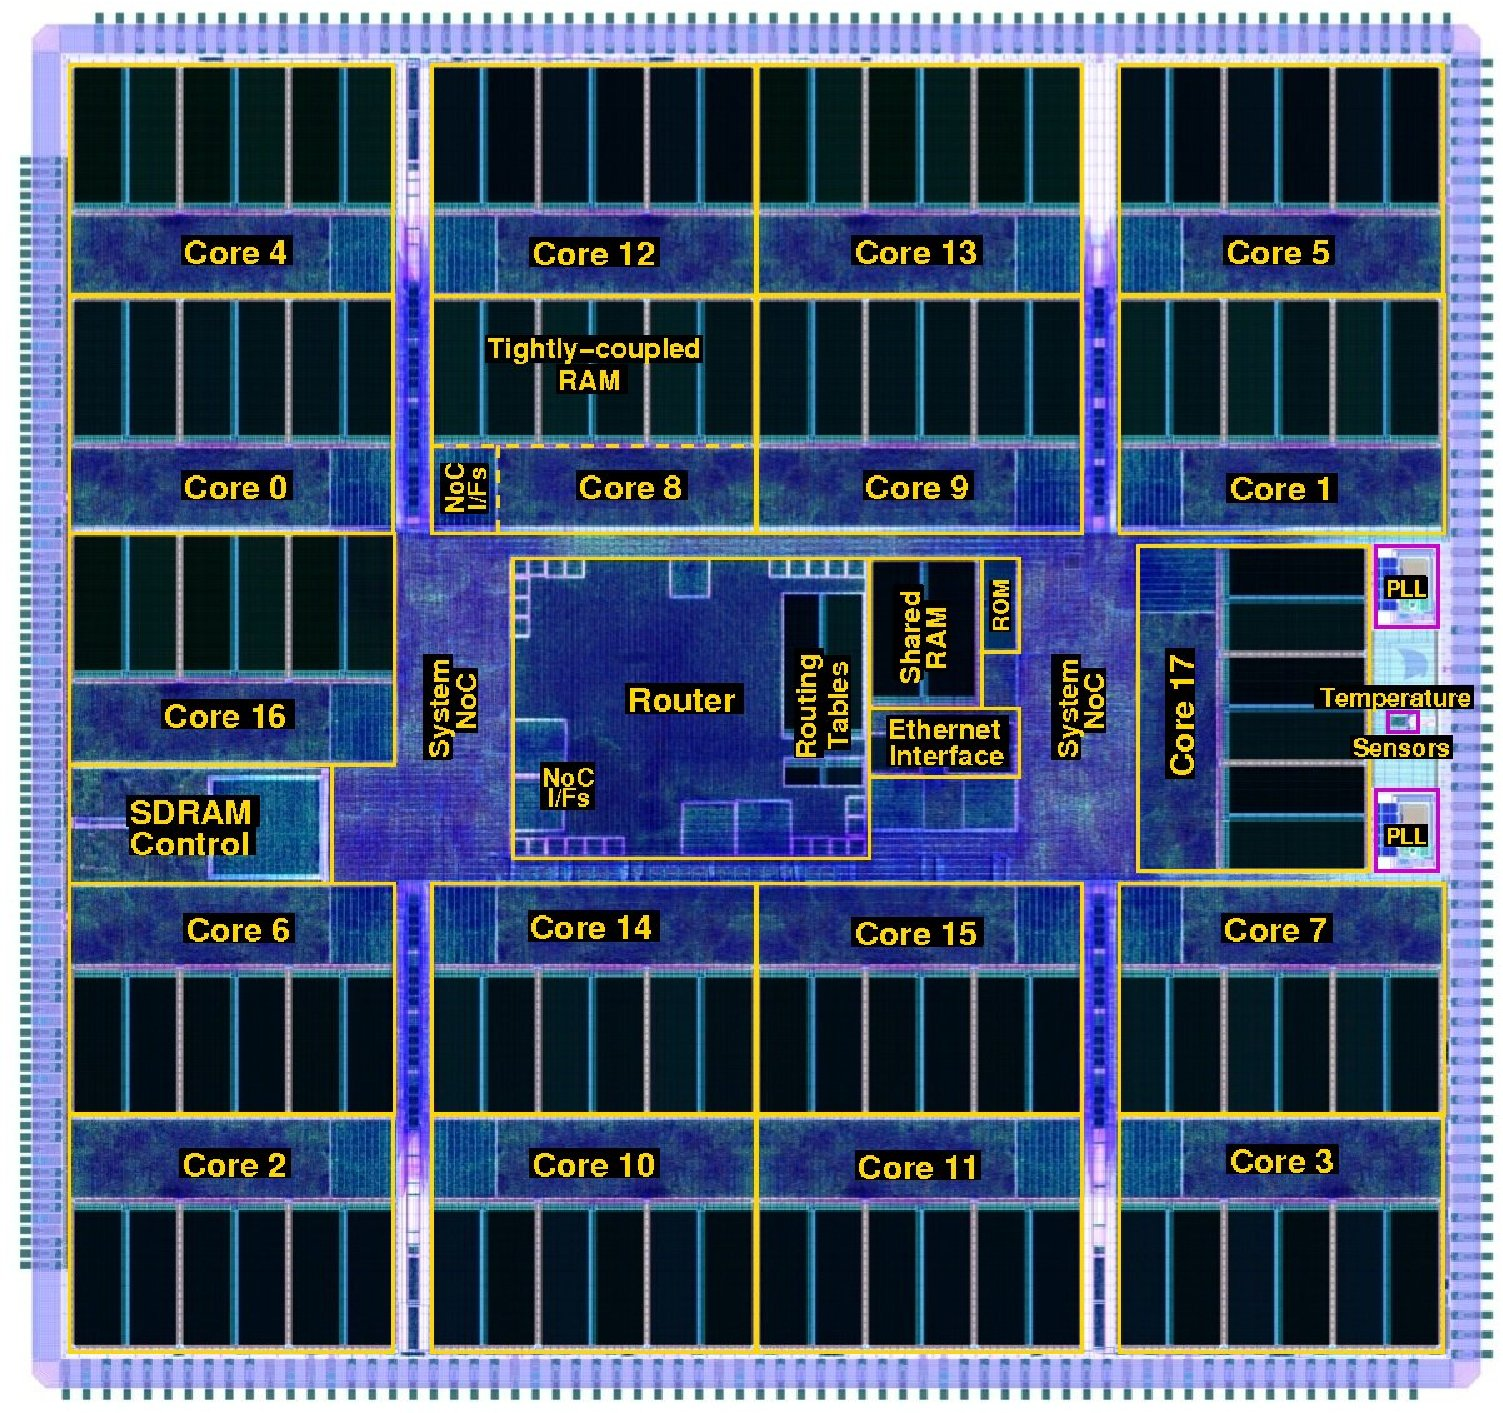
\includegraphics[width=\textwidth]{spinn_labeled_bw}
      \caption{SpiNNaker chip die.}
      \label{fig:hw:spinnaker-die}
    \end{subfigure}
    \hspace*{0.3cm}
    \begin{subfigure}[b]{0.4\textwidth}
      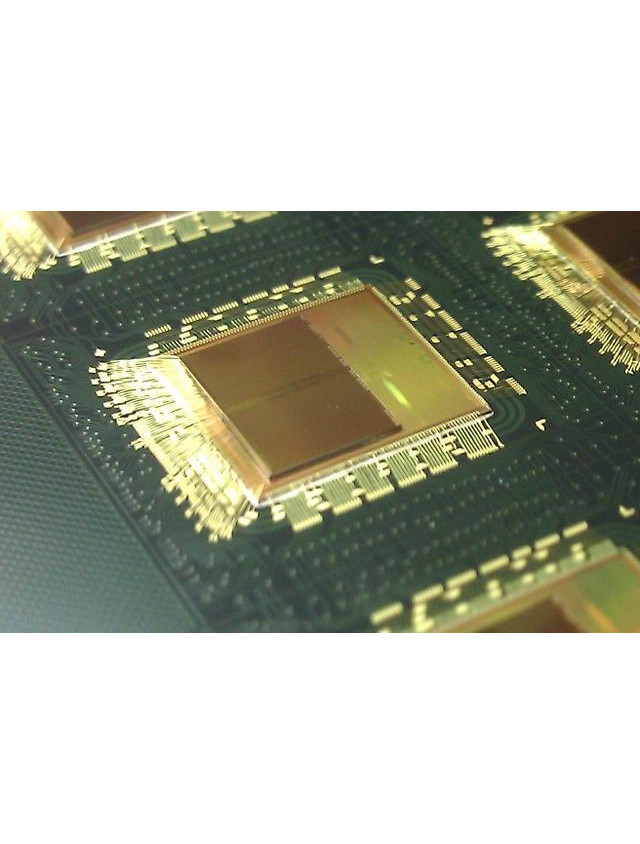
\includegraphics[width=\textwidth]{spinn_dies-ram}
      \caption{Stitch-bonded SDRAM on top of the SpiNNaker chip.}
      \label{fig:hw:bonded-sdram}
    \end{subfigure}
    \caption{SpiNNaker base component, a node, consists of a multi-core chip with stitch-bonded SDRAM.}
  \end{center}
\end{figure}

One of the cores acts as a system controller and, typically, 16 cores will run the applications. Any processor in a chip will have access to four memory spaces. Instruction and data memories are only locally visible (i.e. a core can only see its local memory). These two spaces are composed of a 32 and 64 KByte tightly-coupled blocks of memory, respectively. There are also a 32 KByte block of on-chip SRAM and the 128 MByte off-die SDRAM, both of them are node-local (i.e. seen by all processors in the chip). The cores are able to access the SDRAM using either the System Network-on-Chip (S-NoC) or a DMA controller. No inter-chip memory coherence mechanisms are present~\cite{furber2013overview}.

\subsection{Communications}

One of the notable aspects of the SpiNNaker system is the flexibility of its networking infrastructure. Chips, and therefore cores, have direct links six neighbouring nodes. This provides sufficient connections to form an efficient network that may be configured to form a toroid (Figure~\ref{fig:hw:spinn-toroid}) on a 2D circuit board.

\begin{figure}[h]
  \begin{center}
    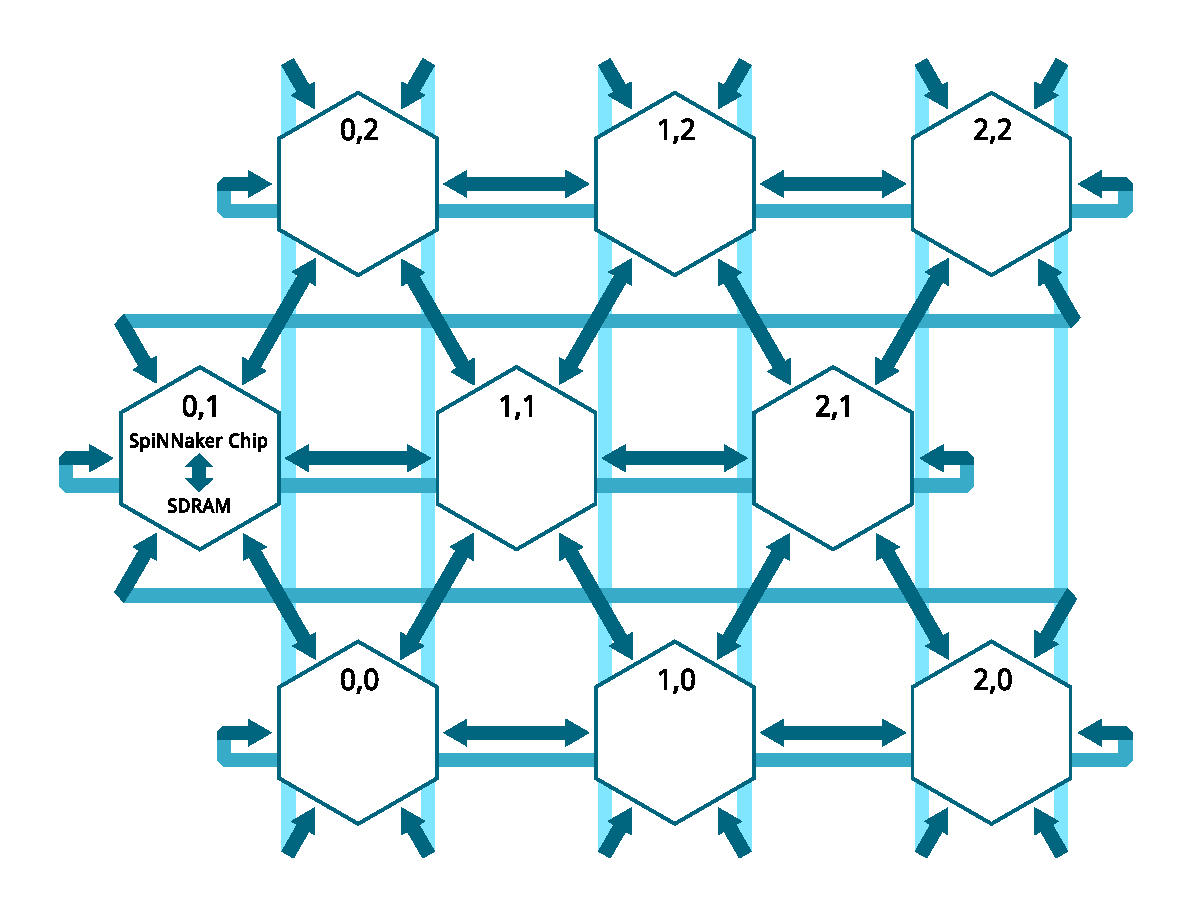
\includegraphics[width=0.7\textwidth]{spinn-interconect}
    \caption{SpiNNaker connected as a toroid.}
    \label{fig:hw:spinn-toroid}
  \end{center}
\end{figure}

Packets are the only way a SpiNNaker chip can communicate to another; a core sends a packet to the local router where it's forwarded to one or more targets. If the target is in the same node, the router will deliver it directly; otherwise, the router sends the packet to an adjacent node where the next router will decide the appropriate move. Packets are either 40 or 72 bit long, a control byte, and one or two 32-bit words.

There are four ways a packet types, each of which are routed differently by the router. Nearest neighbour (NN) and point-to-point (P2P) packets are may be generated by any core, but will only reach the monitor core on the target node. 
Fixed route (FR) packets may be 
The multicast (MC) packet is the only one that permits core-to-core transmission, so applications use this type to transmit data. If the packet has multiple targets, a router along the way will duplicate it and fork the route. This is a highly desired feature for neural applications, since one neuron's axon may connect to multiple neurons dendrites.


\subsection{Programming modes}
Since neurons are thought to react as spikes arrive at their dendrites, SpiNNaker chips support event-based usage.